\section{Extra Credit Question}

\subsection{The Question}

\begin{flushleft}

Re-run question 2, but this time with proper TFIDF calculations
instead of the hack discussed on slide 7 (p. 32).  Use the same 500
words, but this time replace their frequency count with TFIDF scores
as computed in assignment \#3.  Document the code, techniques,
methods, etc. used to generate these TFIDF values.  Upload the new
data file to github.

Compare and contrast the resulting dendrogram with the dendrogram
from question \#2.

Note: ideally you would not reuse the same 500 terms and instead
come up with TFIDF scores for all the terms and then choose the top
500 from that list, but I'm trying to limit the amount of work
necessary.

\end{flushleft}
\subsection{The Answer}


The TFIDF calculation requires the computation of two numbers, the term frequency and the inverse document frequency.
The {\sl term frequency} (TF) is defined as the frequency of the term in the document normalized by the number of terms in the document. 

\begin{center}
\Large
$TF = \frac{\text{number of term occurances}}{\text{number of words in document}}$
\end{center}

The {\sl inverse document frequency} (IDF) of the query is defined as the log base 2 of the number of webpages in the corpus over the number of webpages containing the term. 




\begin{center}
\Large
$IDF =\log_{2} (\frac{\text{number of webpages in corpus}}{\text{number of webpages containing the term}})$
\end{center}


	In the context of the blog matrix this can be visualized easily. Each row consists of a blog vector and each column consists of a term column vector. The elements of the matrix are the occurance frequency of a given term in a specific blog. The code essentially scaled the frequency by the lenght of the blog feed, but that is constant across all terms. The term frequency of a term in a blog is the frequency divided by the number of terms in the blog. In the matrix that is the element value divided by the length of the blog vector. Then summing across all blogs gives the sum of the term frequencies of all blogs which results in a vector of length equal to the number of terms in the corpus. This is the TF value. 	The numerator of the IDF value is constant across all terms and therefore irrelevant. The denominator is the number of blogs that the term appeared it. In matrix view, this represents the number of non-zero elements in a column.
Unfortunately the implementation the book used was not matrix based and therefore some magic had to take place to figure out how to compute these values. However the proper use of dictionaries made the implemention efficient and straight-forward.




\begin{lstlisting}
tf = {}
    blogs = wordcounts
    # go through every blog
    for blog in blogs:
        # go through every term
        for term in blogs[blog]:
            if term in tf: 
                tf[term] += blogs[blog][term]/float(len(blogs[blog])) 
            else:
                tf[term] = blogs[blog][term]/float(len(blogs[blog])) 
    corp = float(len(blogs))
    idf = {}
    for i in apcount:
        idf[i] = log(corp/apcount[i])/log(2)
    tfidf = {}
    for i in tf:
        tfidf[i] = tf[i]*idf[i]
    new = []
    for i in tfidf:
        new.append((i, tfidf[i]))
    new.sort(key=lambda tup:tup[1], reverse=True)
    wordlist = []
    for i in range(500):
        print new[i][0]
        wordlist.append(new[i][0].encode('ascii'))

\end{lstlisting}

The overall accuracy of the two methods is hard to evaluate in an absolute scence because the blogs are not labeled in a way that provides insight to an absolute form of clustering. An attempt to create clusters manually based on the content is not objective and can be easily mislead by our perception of the blogs. Therefore there is no method to score the outcome can then compare the score of the two techniques. 

The one things that does seem to stand out is the distinct tree structure that the two methods display. This become more clear when they are placed alongside each other. The naive term frequency tree seems to randomly split at every iteration. Groupings split up in unequal groups at each step, i.e. a cluster will split up into two clusters, one containing a single blog and then other the rest. This shows that the groups are not very consistent and at the next split the outliers branch off into their own group. This process continues as each cluster loses a blog at each iteration and gets smaller, without any indication of a dictinct seperation into two groups. For example, the food cluster should split up into the desert and the entree clusters, but in this case the food cluster sheds a blog at a time. 

The TFIDF dendrogram appears more structured and precise, very close to binary tree. Throughout the entire process the clusters are divided into subgroups. There are occurances of the random ``one-off'' blog, but that is predictable. Also, the number of terms used is only 500, which many not be large enough to provide a proper result.  The TFIDF method appear to find dominant characteristics of the cluster to patition on. While the naive method finds the most eccentric member and removes him. 

One a more abstract, and slightly ``hand-wavy'', interpretation blogs represent the people that write them. A population can be clusters into in a variety of ways, i.e. hobby, occupation, gender, age, but the clusters that provide the most information are the ones that partition the cluster into the subgroups that are bound by a characteristic. This type of clustering is equivalent to a useful demographic map, e.g. young male engineers, young female engineers, retired wood craftsman, etc. The group can be used to describe its members in a reasonable way. However, the population can be clustered based on who is a Harvard graduate that is also in an underground alt-rock band and not.  There is lots of detail about one group, but there members of the other group are not held together by any common traits.  Adolf Hitler and Edward Snowden would be in the same cluster and then the question become what do they have in common. 
\begin{figure*}[t!]
        \centering
        \begin{subfigure}{0.5\textwidth}
	\centering
	 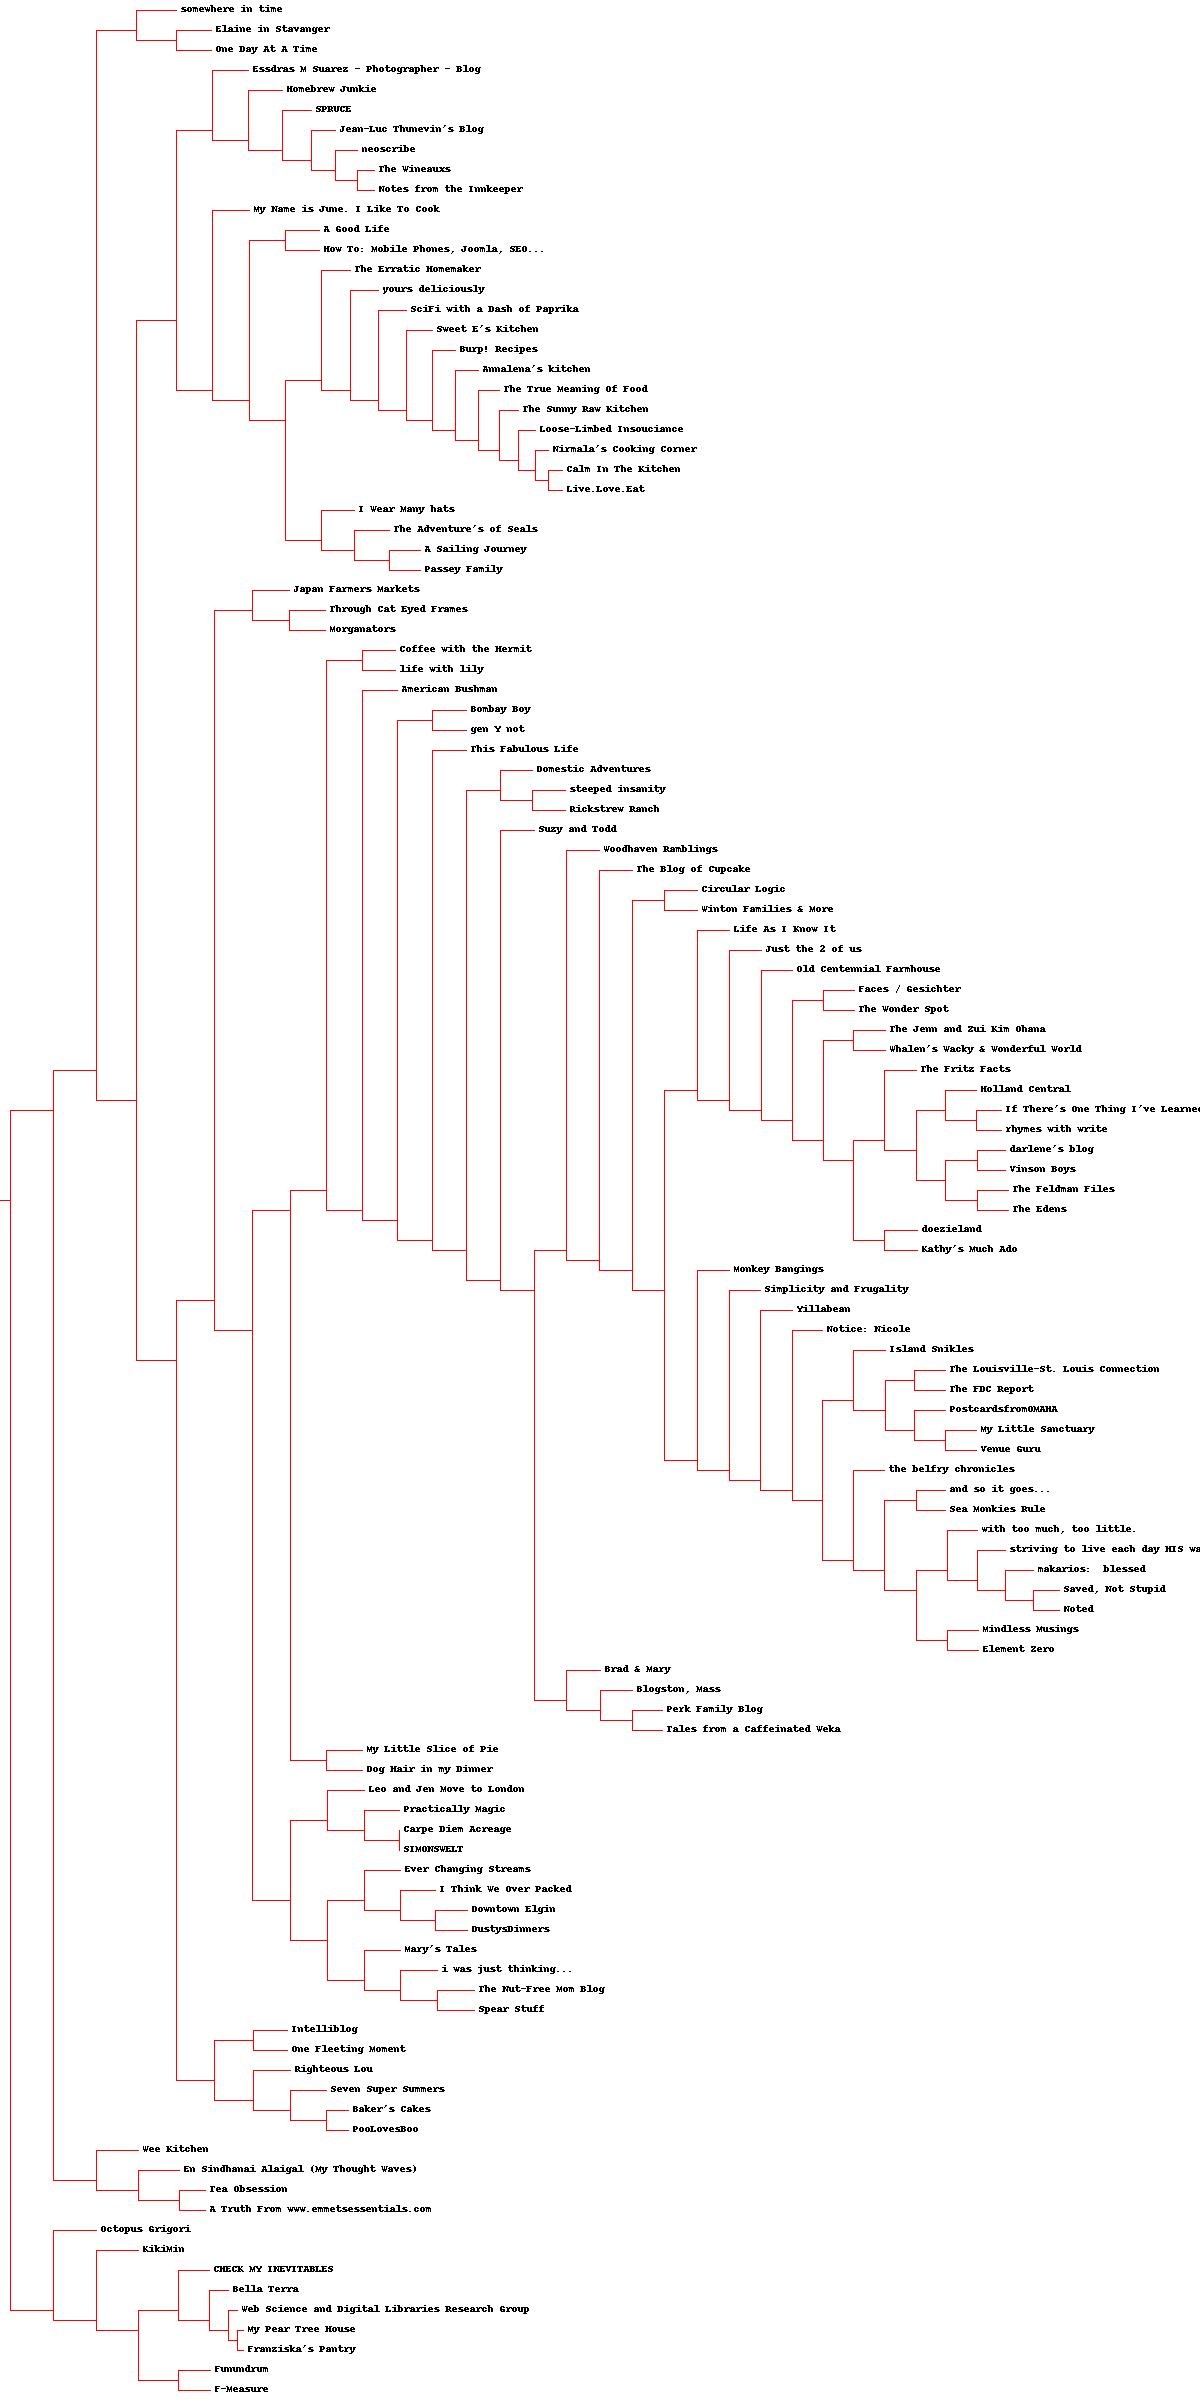
\includegraphics[height=11cm, width=9cm]{../q2/blogdendro.jpg}

             \caption{Dirty Hack}
        \end{subfigure}%
        \begin{subfigure}{0.5\textwidth}
		\centering
               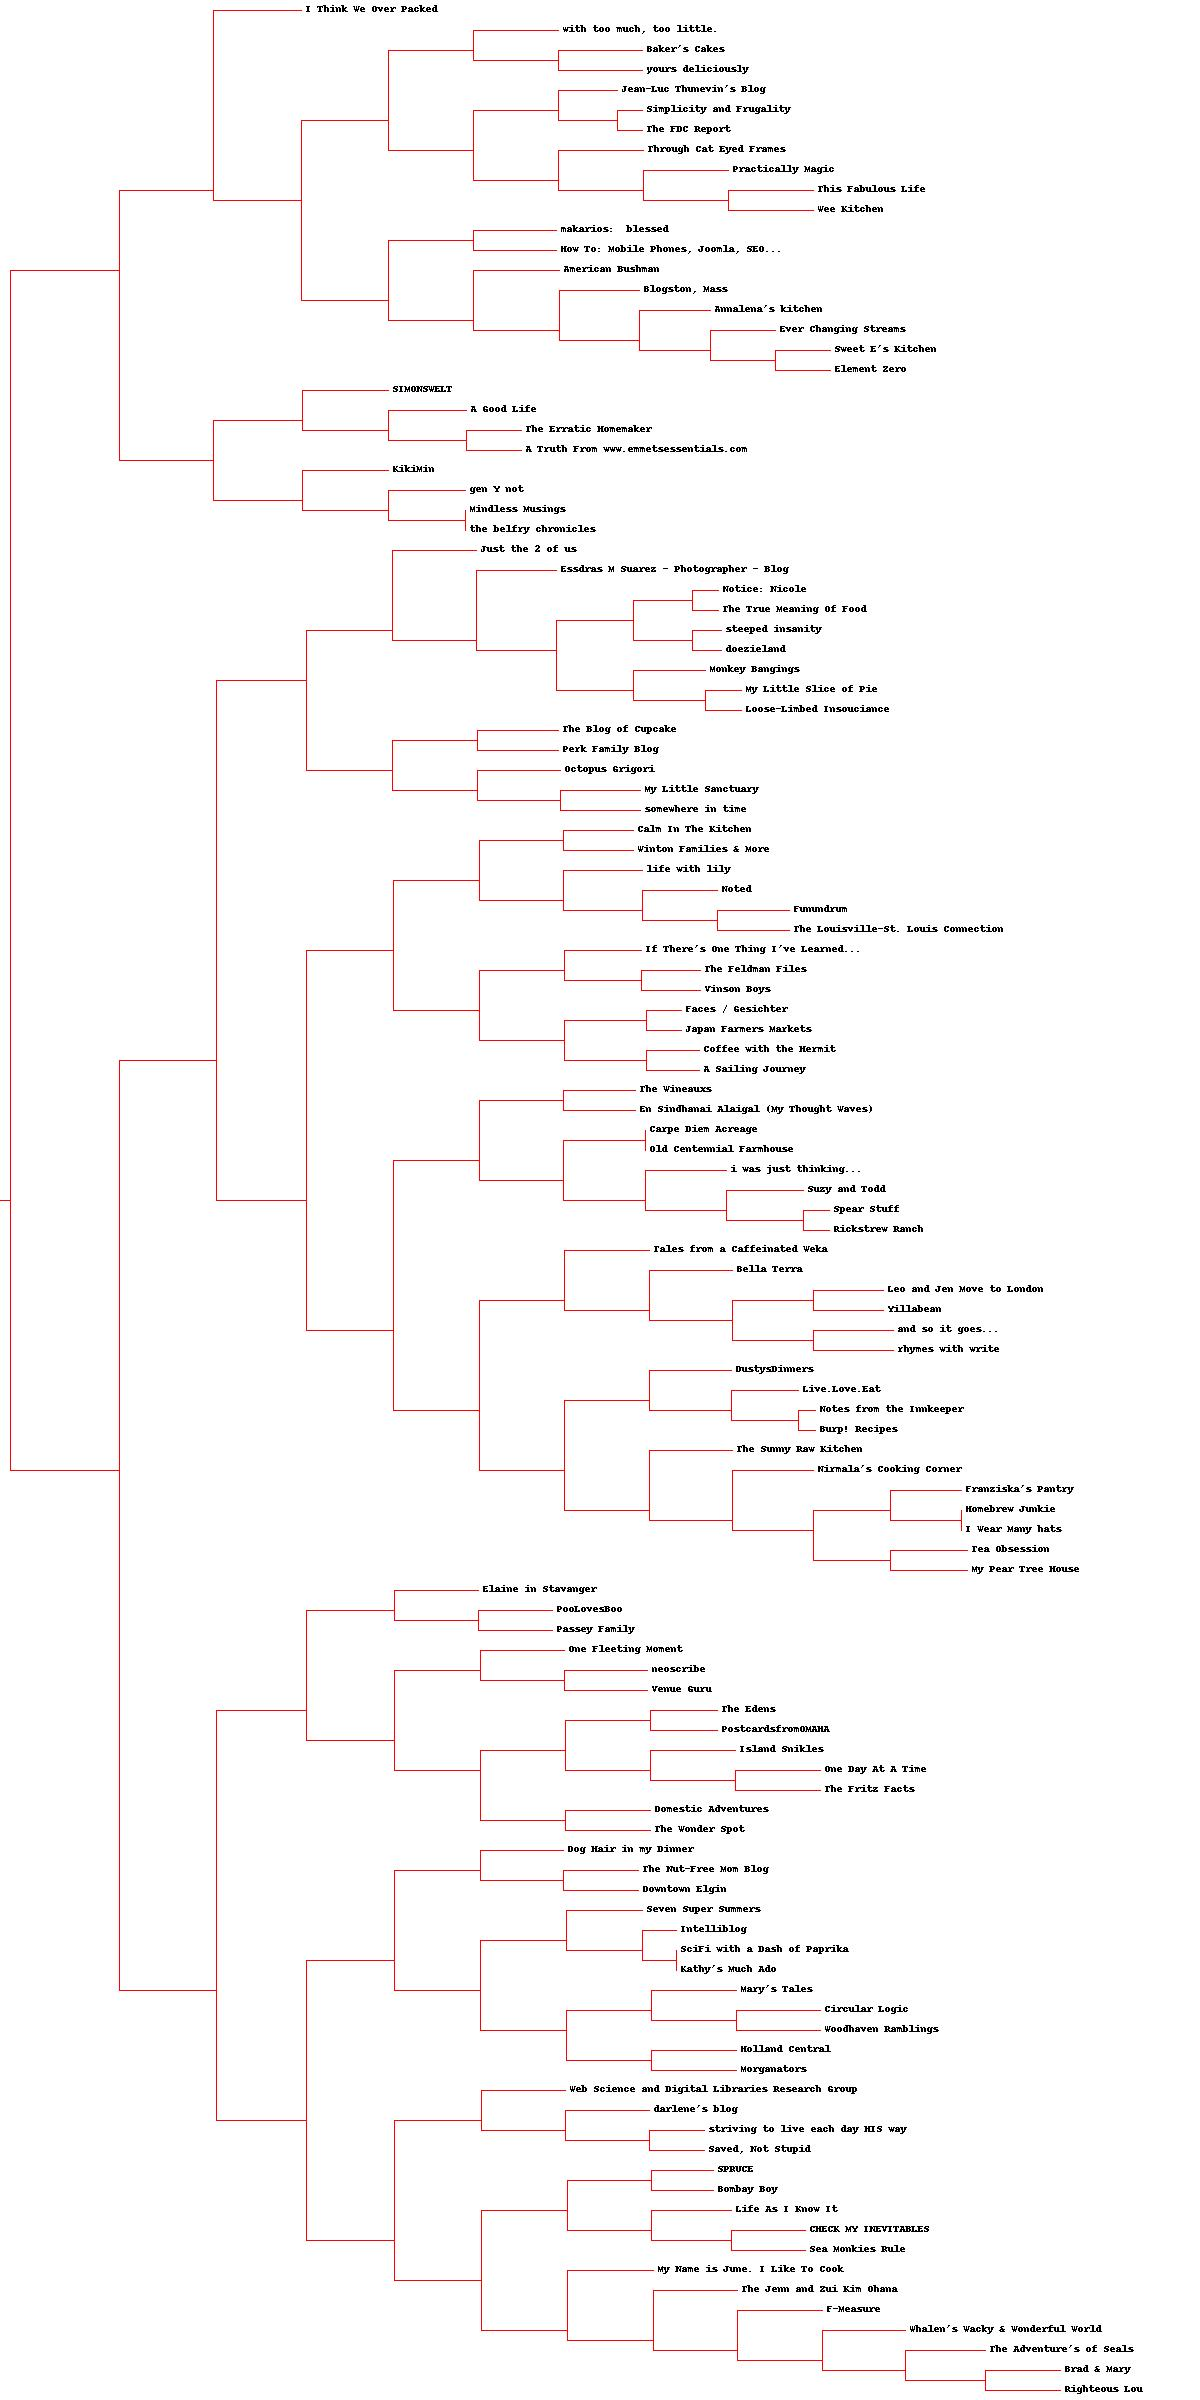
\includegraphics[height=11cm, width=9cm]{../qec/blogdendro}	
\caption{TFIDF}
        \end{subfigure}
    
\end{figure*}



In conclusion, my opinion is that the TFIDF measure clusters in a way that produces distinct subgroups which are meaningful and consistent. On the other hand, the naive approach partitions based on the odd one out, but sometime the odd one isnt very odd and the non-odd ones dont have much to do with each other. This is the conclusion that I draw based on the structure of the divisions. Even if the groups don't seem related based on the title they have some common characteristic that TFIDF can determine, but the naive method does not.








\begin{figure}[h!]
\centering
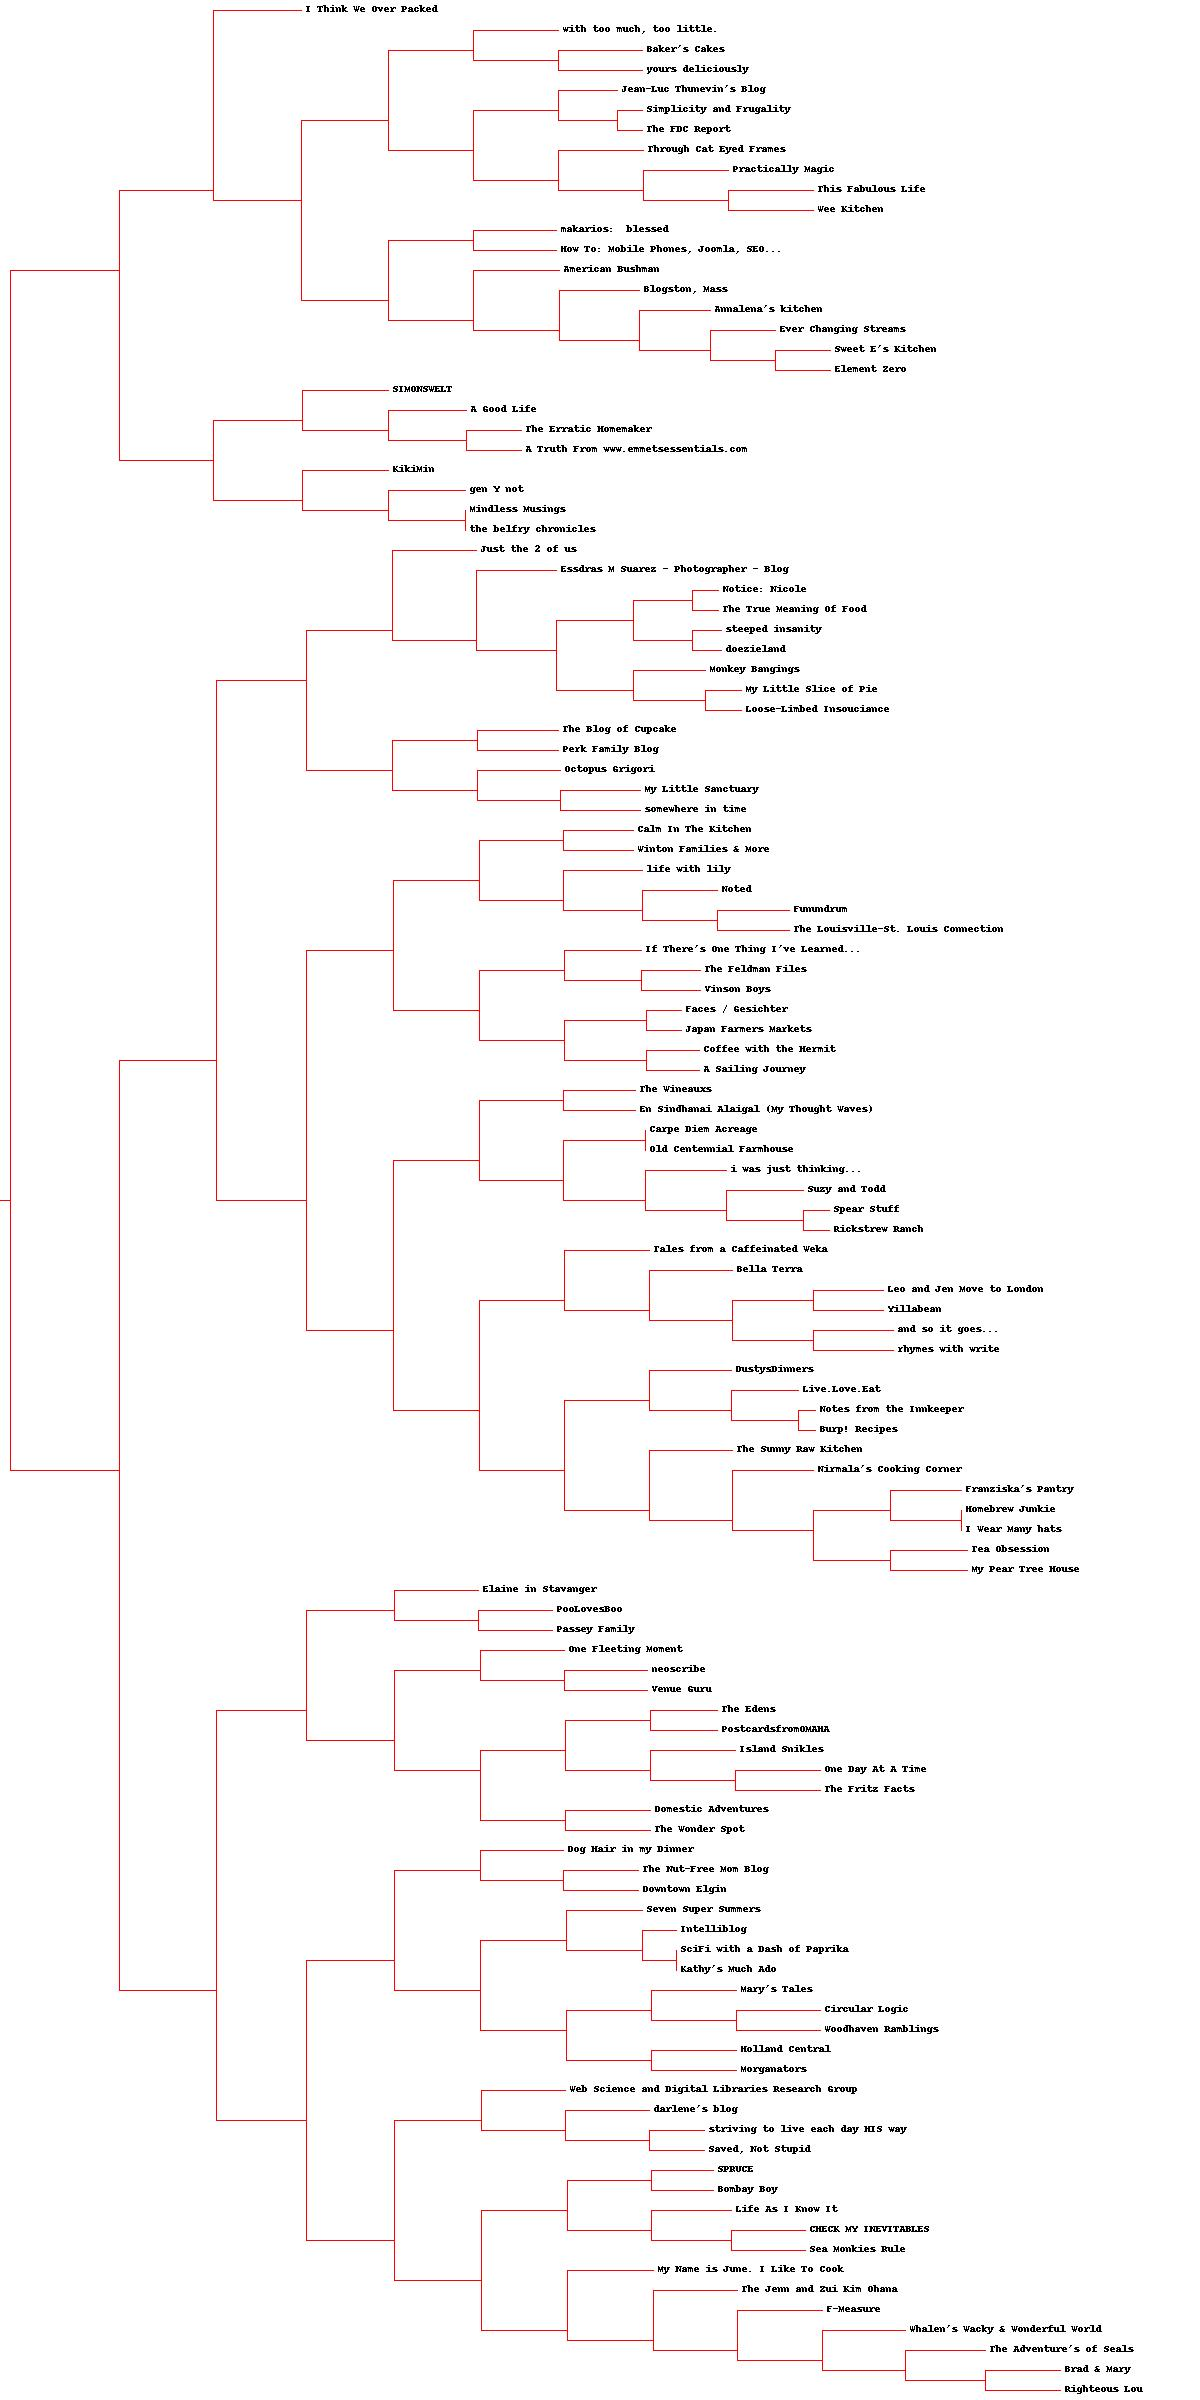
\includegraphics[height=25cm]{../qec/blogdendro}
\caption{TFIDF dendrogram}
\end{figure}






